\chapter{Evaluation protocol details}
\label{app:protocol}

\section{Prompt for live-model transcription}
\label{app:prompt}

\begin{verbatim}
Write down the words spoken in this audio, exactly as spoken.

If no words are audible, leave the transcript empty and set status to no_speech.
\end{verbatim}


\section{Pinned components of the measuring instrument}
\label{app:pinned}

% TODO: complete the judge row once selected. Every judge result must record
% the exact model identifier, the exact prompt, the input modality and the run
% date, because closed models change without notice.

\begin{table}[h]
  \mytable
  \begin{tabularx}{\textwidth}{@{}lL@{}}
    \toprule
    Component & Identity \\
    \midrule
    Text normaliser        & \texttt{whisper-normalizer} 0.1.15, \texttt{EnglishTextNormalizer} \cite{whisper_normalizer,radford2023whisper} \\
    Baseline transcriber   & \texttt{faster-whisper} 1.2.1, \texttt{small.en}, int8 quantisation, greedy decoding \cite{faster_whisper,radford2023whisper} \\
    Word error rate        & \texttt{jiwer} 4.0.0 \cite{jiwer} \\
    Stopword list          & \texttt{NLTK} English stopwords \cite{bird2009nltk}, snapshotted into the source tree so the list cannot change with a library upgrade \\
    Judge model            & \emph{to be recorded} \\
    Random seed            & 42 \\
    \bottomrule
  \end{tabularx}
  \caption{Components of the evaluation instrument, pinned by version. A change
           to any row invalidates comparison with numbers reported before it.}
  \label{tab:pinned}
\end{table}


\chapter{Room construction}
\label{app:rooms}
\label{sec:room_construction}

Each trial is rendered in its own simulated room rather than convolved with a
recorded impulse response, so that the acoustics are a controllable variable
rather than a property of whichever room happened to be recorded. Rooms are
rectangular (``shoebox'') and the impulse responses are generated by the
image-source method using \texttt{pyroomacoustics} 0.10.1
\cite{scheibler2018pyroomacoustics}.

For every trial the renderer draws the room's three dimensions, a reverberation
time, and independent positions for the microphone and the two talkers. Wall
absorption is not drawn directly: it is solved for from the requested
reverberation time and the room's surface area by the Sabine relation, and the
draw is rejected and retaken if the combination is not physically realisable.
Both talkers are placed in the same room and share the microphone, so the two
speech signals arrive with different but consistent room responses.

\begin{figure}[H]
  \centering
  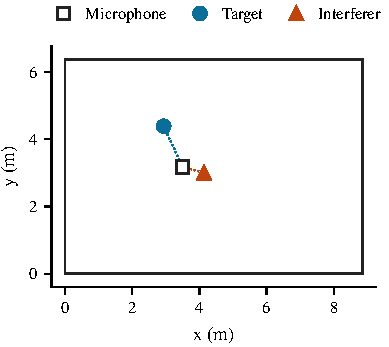
\includegraphics[width=0.4\textwidth]{figures/room_example_a.pdf}
  \caption{Plan view of the room rendered for trial \texttt{train-42-007495}. The room measures $8.85 \times 6.38 \times \SI{3.14}{\metre}$ (\SI{177}{\cubic\metre}) with a reverberation time of \SI{0.250}{\second}, for which the Sabine relation gives a wall absorption of \num{0.5479}. The microphone sits at $(3.50, 3.18, 1.28)$~m, the target at $(2.94, 4.39, 1.66)$~m and the interferer at $(4.14, 3.00, 1.57)$~m, placing them \SI{1.39}{\metre} and \SI{0.72}{\metre} from the microphone respectively.}
  \label{fig:room_a}
\end{figure}

\begin{figure}[H]
  \centering
  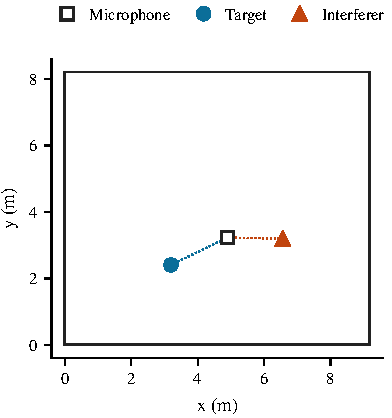
\includegraphics[width=0.4\textwidth]{figures/room_example_b.pdf}
  \caption{Plan view of the room rendered for trial \texttt{train-42-004785}, the most reverberant in the split. The room measures $9.18 \times 8.21 \times \SI{3.48}{\metre}$ (\SI{263}{\cubic\metre}) with a reverberation time of \SI{0.600}{\second}, for which the Sabine relation gives a wall absorption of \num{0.2594} which is less than half that of \autoref{fig:room_a}, in a room \SI{49}{\percent} larger. The microphone sits at $(4.91, 3.23, 1.49)$~m, the target at $(3.20, 2.40, 1.52)$~m and the interferer at $(6.56, 3.19, 1.64)$~m, placing them \SI{1.90}{\metre} and \SI{1.67}{\metre} from the microphone respectively.}
  \label{fig:room_b}
\end{figure}


\chapter{Construction parameters}
\label{app:params}

Every parameter below is drawn independently per trial from the stated distribution, except where a regime overrides it. Ranges written $[a, b]$ are sampled uniformly on that interval.

\begin{table}[h]
  \mytable
  \begin{tabularx}{\textwidth}{@{}llL@{}}
    \toprule
    Parameter & Distribution & Meaning \\
    \midrule
    \multicolumn{3}{@{}l}{\emph{Trial layout}} \\
    Mixture length        & $[15.0, 20.0]$ s   & Duration of the rendered trial \\
    Overlap ratio         & $[0.0, 0.7]$       & Fraction of target speech with the interferer also talking \\
    Overlap tolerance     & $0.03$             & Accepted deviation from the requested overlap \\
    Target activity ratio & $[0.15, 0.78]$     & Fraction of the trial in which the target speaks \\
    Activity tolerance    & $0.1$              & Accepted deviation from the requested activity \\
    Utterances per source & $\le 6$            & Cap on how many utterances one recording may contribute \\
    \midrule
    \multicolumn{3}{@{}l}{\emph{Levels}} \\
    SIR                   & $[-5.0, 15.0]$ dB  & Target loudness relative to the interferer \\
    SNR                   & $[0.0, 20.0]$ dB   & Target loudness relative to the noise bed \\
    Target loudness       & $[-33.0, -25.0]$ LUFS & Absolute level of the target, BS.1770 integrated \cite{itu2015bs1770} \\
    Clip ceiling          & $0.95$             & Peak after which the whole trial is rescaled together \\
    \midrule
    \multicolumn{3}{@{}l}{\emph{Room}} \\
    $T_{60}$              & $[0.25, 0.6]$ s    & Reverberation time \\
    Room length, width    & $[5.0, 10.0]$ m    & Floor plan \\
    Room height           & $[3.0, 4.0]$ m     & \\
    Source distance       & $[0.1, 2.0]$ m     & Talker to microphone \\
    Source height         & $[0.9, 1.8]$ m     & Talker, seated to standing \\
    Microphone height     & $[0.9, 1.8]$ m     & \\
    Early reflections     & $50$ ms            & Cutoff separating early echoes from the late tail \\
    \midrule
    \multicolumn{3}{@{}l}{\emph{Enrolment}} \\
    Enrolment length      & $5.0$ s            & Single clip, levelled, carrying no room \\
    EQ augmentation       & $p = 0.5$          & Three peaking biquads, log-uniform \SIrange{120}{6400}{\hertz}, $\pm$\SI{6}{\decibel}, $Q = 1.0$, RMS restored \\
    \midrule
    \multicolumn{3}{@{}l}{\emph{Speaker pairing}} \\
    Same-gender fraction  & $0.5$              & Proportion of trials whose two talkers share a gender \\
    \midrule
    \multicolumn{3}{@{}l}{\emph{Speech detection} \cite{silero2021vad}} \\
    Silence threshold     & $250$ ms           & Pause length after which a talker counts as stopped; \textbf{this defines overlap} \\
    Speech probability    & $0.5$              & Frame-level threshold \\
    Minimum speech        & $100$ ms           & Shortest run counted as speech \\
    Speech padding        & $30$ ms            & Added either side of a detected run \\
    Noise-bed rejection   & $0.5$ s            & Longest run of detected speech tolerated in a WHAM! clip \\
    \midrule
    \multicolumn{3}{@{}l}{\emph{Regimes}} \\
    Regime weights        & $0.6$ / $0.4$      & Proportion of trials drawn as \texttt{base} / \texttt{hard} \\
    \texttt{base} SIR     & $[0.0, 12.0]$ dB   & Regime override \\
    \texttt{base} SNR     & $[8.0, 20.0]$ dB   & Regime override \\
    \texttt{base} activity & $[0.45, 0.78]$    & Regime override \\
    \texttt{base} $T_{60}$ & $[0.25, 0.5]$ s   & Regime override \\
    \bottomrule
  \end{tabularx}
  \caption{Construction parameters and their sampling distributions.}
  \label{tab:params}
\end{table}

